\documentclass[a4paper]{article}

\usepackage{a4}
\usepackage[utf8]{inputenc}
\usepackage[french]{babel}
\usepackage[T1]{fontenc}
\usepackage{graphicx}
\usepackage{amsmath}
\usepackage{amssymb}
\usepackage{float}

\DeclareUnicodeCharacter{2212}{-}
\author{Igor et Jean}
\date{\today}
\title{Synthèse mathématiques}
\parskip=5pt
\begin{document}
    \maketitle
    \tableofcontents
    \section{Étude de fonction}

    \subsection{Introduction}
    Une fonction prend une valeur $x$ en \emph{fonction} de laquelle elle
    retourne une valeur y. On peut alors faire un graphique de la fonction avec,
    en ordonnée, la valeur retournée et, en abscisse, la valeur insérée. 

    \textbf{Exemple d'une fonction}
    \begin{equation}\label{eq:fct1d}
       f(x) = ax + b 
    \end{equation}

    \subsection{Premier degré}\label{ss:pd}
    La fonction \ref{eq:fct1d} est du premier degré. On le remarque par son
    équation dont l'élément le plus élevé est du premier degré. Ainsi, on dit
    d'une fonction qu'elle est du degré de son élément le plus élevé.

    La \emph{pente} caractérise l'inclinaison de la droite ; la différence dans
    le changement de $x$ et $y$. Un changement égale produit un angle de 45° et
    une pente de 1.

    \begin{equation}\label{eq:pente1}
        pente = \frac{y_1 - y_2}{x_1 - x_2}
    \end{equation}

    Deux droites sont perpendiculaires si leurs pentes sont inverses et opposées
    et son parrallèles si leurs pentes sont identiques.

    Pour trouver l'équation de la droite qui passe par deux points, il faut
    trouver la pente de la droite à l'aide de l'équation \ref{eq:pente1} puis,
    pour trouver b, mettre un des deux points dans l'équation.

    Pour trouver le point d'intersection de deux fonctions, il faut fusionner
    leurs équations en une, et résoudre pour trouver $x$.  Celui-ci,
    correspondant à la valeur en abscisse du point, on peut trouver $y$ en
    l'implémentant ($x$) dans l'équation.
    
    \subsection{Deuxième degré (à une inconnue)}
    Une fonction du deuxième degrés peut toujours s'écrire sous la forme
    
    \begin{equation}\label{eq:ddbase}
    f(x) = ax^2 + bx + c
    \end{equation}

    Vu que $x$ est la seule inconnue, $a$, $b$ et $c$ sont définis.

    On peut trouver la/les valeures de $x$ qui font en sorte que la fonction
    retourne $0$ grâce à l'équation suivante.

    \begin{equation}\label{eq:resdds}
        x = \frac{{}-b \pm \sqrt{b^2 -4ac}}{2a} 
    \end{equation}

    \noindent Ces valeurs sont appelées \underline{racines}. Il peut y en
    avoir aucune, une ou deux.

    La partie dans la racine carrée est appelée le \underline{delta} ($\Delta$). 

    Comme toutes les fonctions, on peut les représenter graphiquement ; une
    parabole pour celle du deuxième degré.
    \begin{figure}[H]
        \centering
        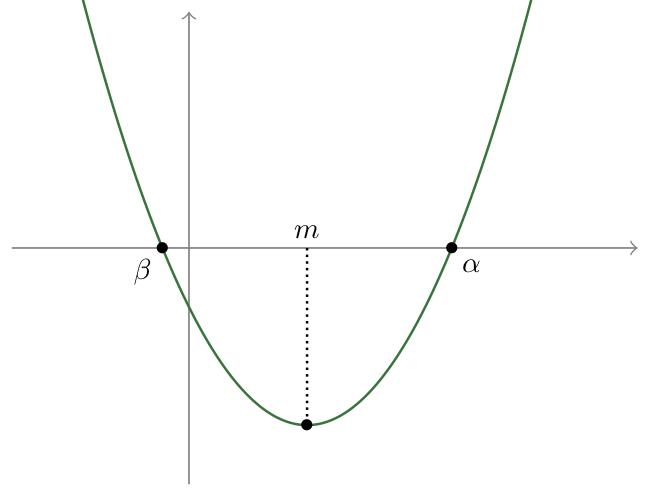
\includegraphics[scale=0.3]{parabole.png}
        \caption{Graphique d'une fonction du deuxième degré}
        \label{fig:parabole}
    \end{figure}

    Une fonction du deuxième degré n'a besoin que de trois paramètres pour
    être définie. Celles-ci sont illustrée sur la figure \ref{fig:parabole} par
    $\alpha $, $\beta $ et $m$

    $\alpha$ et $\beta$, sont les valeurs qui touchent l'axe des abscisse ; qui
    retournent $0$. Ce sont, comme on la vu ci-dessus, les racines et peuvent
    être calculée par le biais de l'équation \ref{eq:resdds}.
    
    Quand la fonction n'a pas de racine, dans le cas où delta ($\Delta$) est 
    negatif, la parabole ne touche pas l'axe des abscisses. Quand la fonction
    n'a qu'une racine, le delta égale $0$ et la courbe ne touche l'axe qu'une 
    fois. Dans le cas où le delta est positif, la fonction a deux racine et
    touche deux fois l'axe comme dans la figure \ref{fig:parabole} ci-dessus.

    $m$ est le sommet de la fonction. Celle-ci peut-être calculée avec grâce
    à l'équation 

    \begin{equation}
        m = \frac{-b}{2a}    
    \end{equation}

    Une fonction $f(x) = ax^{2}+bx+c$ dont les racines sont $\alpha$ et $\beta$
    peut être factorisée en 
    \begin{equation}\label{eq:ddfact}
    a(x - \alpha)(x - \beta)
    \end{equation}

    \noindent car ses racines et son sommet, les seuls paramètres définissant,
    seront les mêmes.

    Rajouter trouver forme gràce à a, b avec en outre.

    \subsection{Troisième, quatrième degré, etc}
    \begin{figure}[H]
        \centering
        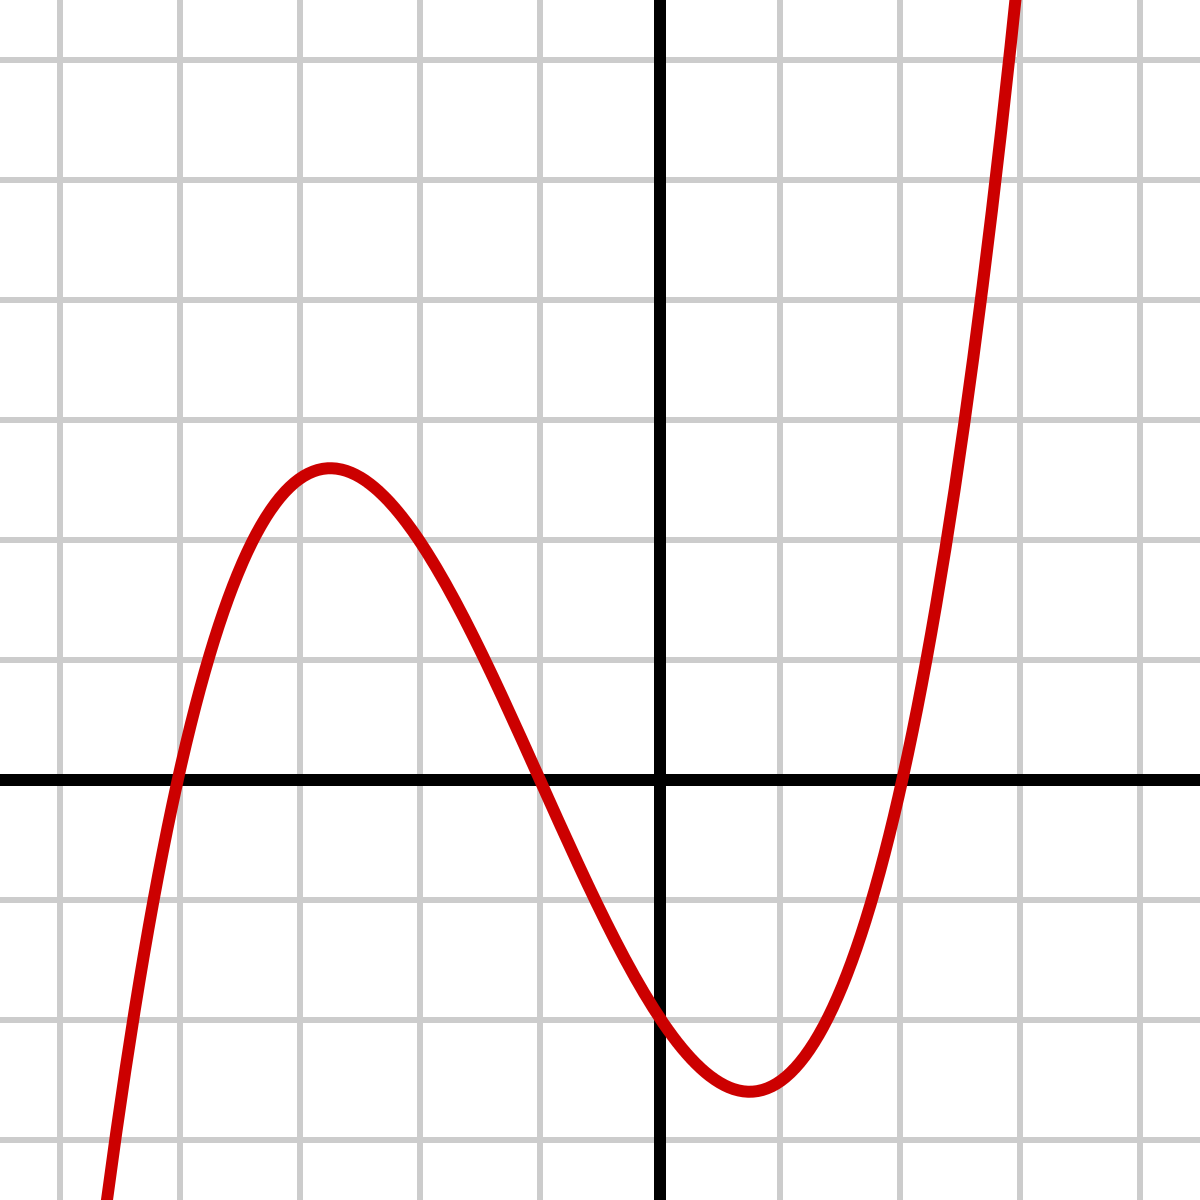
\includegraphics[width=0.49\textwidth, height=100pt]{3d.png} 
        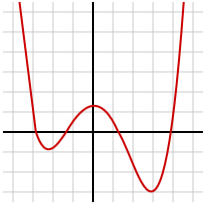
\includegraphics[width=0.49\textwidth, height=100pt]{4d.png} 
        \caption{Courbe du 3ème et 4ème degré}
        \label{fig:34d}
    \end{figure}

    Les fonctions qui ont un degré supérieur à 1 sont représentée par
    des courbes ayant au maximum un sommet et toujours deux changements de
    concavité en moins que le degré. 
    

    Les courbes de degrés pairs ont les deux extrêmes pointant dans la même
    direction (haut si $a$ est positif, bas dans le cas contraire). Les
    fonctions de degrés impairs ont les deux extrêmes qui pointes dans des
    directions opposées (si $a$ est positif, la gauche pointe vers le bas, sinon
    inverse).

    \subsection{dérivées}
    La dérivée d'une fonction est une autre fonction (courbe ou droite) qui
    représente sa pente pour chaque point donné (en $x$). La pente, comme vu
    dans la partie \ref{ss:pd}, est l'ampleur du changement de la proportion,
    entre la valeur retournée ($y$) et la valeur d'entrée ($x$).

    La dérivée est une fonction d'un degré en moins. Ainsi, la pente d'une
    fonction du deuxième degré varie linéairement, celle d'une fonction du
    troisième degré varie selon un parabole et ainsi de suite.

    Quand la dérivée (pente) est positive, la courbe monte. Quand elle est
    négative, la courbe descend. Quand elle est à $0$, qu'elle change de
    signe, on se trouve à un sommet.

    Pour trouver la pente d'une courbe, il faut comparer deux points infinement
    proches, car au plus les points sont proches, au plus la courbe semble
    linéaire et le pente est précise. 

    La pente en un point $x$ est de 

    \begin{equation}\label{eq:derivbase}
        \lim_{\delta \to 0} \frac{f(x + \delta ) - f(x)}{\delta}
    \end{equation}
    \noindent Car la pente est la variation de $y$ par rapport à $x$, et ici,
    $x$ correspond à $\delta$. En levant la limite, on peut trouver l'équation
    de la dérivée.

    A partir de cette règle, on peut trouver que pour dériver $f(x)$, il faut
    appliquer la règle suivante sur chaqu'un de ses éléments 

    \begin{equation}\label{eq:derivutil}
        (x^{n})' = n \cdot x^{n - 1}
    \end{equation}
    \noindent Ici, $x^n$ représetente un élément de la fonction, $x$ étant
    l'inconnu \emph{et} son facteur (ainsi, le facteur est aussi multiplié par
    $n$). 
    

    L'élément élevé au premier degré se transforme en $1$, donc on ne garde que
    son facteur.

    L'élément $c$ (voire dans l'équation \ref{eq:ddbase}) n'est, à première vue,
    pas associé à $x$. Pour l'implémenter dans l'équation, on peut se le
    représenter comme $c \cdot x^0$. Donc, il sera toujours égal à 0.

    Voici d'autres formules sur l'algèbre des dérivée. 

    \begin{align}
        &(\lambda \cdot f(x))' = \lambda \cdot f(x)' \label{eq:de1}\\
        &(f(x) + g(x))' = f'(x) + g'(x) \label{eq:de2}\\
        &(f(x) - g(x))' = f'(x) - g'(x) \label{eq:de3}\\
        &(f(x) \cdot g(x))' =  f'(x) \cdot g(x) +  f(x) \cdot g'(x)
        \label{eq:de4}\\
        &(f^n(x))' = n \cdot f'(x) \cdot f^{n-1}(x) \label{eq:de5}\\
        &(\frac{f(x)}{g(x)})= \frac{f'(x) \cdot g(x) - f(x) \cdot g'(x)}{g^2(x)}
        \label{eq:de6}
    \end{align}


    Celle-ci donne une idée de la vitesse à laquelle la pente évolue et dans
    qu'elle direction ; si elle accèlère ou freine.

    Ainsi, elle nous donne une idée de la concavité de la courbe alors que
    la dérivée première ne nous donne que la direction.
    
    \subsection{Domaines et asymptotes}
    Dans une fonction, pour chaque entrée, on n'a qu'une seule valeur
    correspondante. \underline{L'image} d'une fonction regroupe toutes les
    valeurs qu'elle peut retourner ; qu'elle sait atteindre.

    À l'inverse, le \underline{domaine} regroupe tous les nombres (entrées) pour
    lesquels une valeure existe. Pour voir comment on définis un ensemble de
    nombres, aller à la partie \ref{ss:jargondom}.

    Le domaine d'une fonction correspond généralement à tous les nombres réels.
    Toutefois, si celle-ci contient une inconnue dans une racine carrée ou au
    dénominateur, le domaine peut varier.


    \subsection{Analyse et tableau de signe}
    \subsection{Exemple d'une étude}
    \section{Nombres complexes}
    \section{Les groupes} 
    Un groupe est un ensemble $E$ auquel est associé une opération (binaire)
    $\star$ vérifiant les lois \ref{eq:gr1}, \ref{eq:gr2}, \ref{eq:gr3} et
    \ref{eq:gr4}.

    \begin{align}
        &\forall \ a, b \in E, \ a \star b \in E \label{eq:gr1}\\
        &(a \star b) \star c = a \star (b \star c)\label{eq:gr2} \\
        &\exists \ e \in E : a \star e  = e \star a = a \ \ \ \forall a \in E
        \label{eq:gr3}\\
        &\forall a \in E, \exists a^{-1} \in E : a \star a^{-1} = a^{-1} \star a
        = e \label{eq:gr4}
    \end{align}

    Ci dessus, la loi \ref{eq:gr1} est la \underline{loi de composition
    interne}. Elle indique que l'opération éffectuée deux nombres quelconques de
    l'ensemble retourne toujours un autre nombre de l'ensemble. 

    La loi \ref{eq:gr2} est celle de \underline{l'associativité} et indique
    que l'opération binaire peut être faite dans n'importe qu'elle ordre.

    La loi \ref{eq:gr3} exprime la présence d'un \underline{neutre}. Le
    neutre est un élément appartenant à l'ensemble qui laisse les éléments
    composés avec lui inchangés. Par exemple, le neutre de l'addition est $0$
    car $a + 0 = a$. Le neutre de la multiplication est $1$ car $a \cdot 1 = a$

    Finalement, la loi \ref{eq:gr4} énonce la présence d'\underline{inverses},
    appartenant à l'ensemble, pour chaque élément de l'ensemble. Par definition,
    la composition d'un nombre et de son inverse retourne le neutre. Par
    exemple, dans le cas de l'addition, l'inverse de $a = -a$ car $a + (-a) = 0$
    qui est le neutre. Pour la multiplication, l'inverse de $a = \frac{1}{a}$
    car $a \cdot \frac{1}{a} = \frac{a}{a} = 1$ étant le neutre. 

    Les nombres entiers $\mathbb{Z}$ munis de l'addition (+) forment un groupe.
    L'ensemble des nombres rationnels $\mathbb{Q}$ et la multiplication ne forme
    pas un groupe car il n'obéit pas à la règle \ref{eq:gr4} si $a = 0$. Il
    n'existe pas de nombre rationnel qui transforme un 0 en neutre (1).

    Quelques autres exemples :
    \begin{itemize}
        \item $\mathbb{N}, +$ n'est pas un groupe car il n'y a pas d'inverse.
        \item $\mathbb{Z}, \cdot $ n'est pas un groupe.
        \item $\mathbb{Q}, +$ est un groupe.
        \item $\mathbb{R}, +$ est un groupe.
        \item $\mathbb{R}, \cdot$ n'est pas un groupe.
        \item $\mathbb{R}_0, \cdot$ est un groupe.

    \end{itemize}
    
    On dit d'un groupe qu'il est \underline{commutatif/abélien} s'il répond à la
    loi
    \begin{equation}
        \forall a, b \in E : \ \ a \star b = b \star a
    \end{equation}
    
    Les \underline{symétries} d'un objet correspond aux actions qui, opérées sur
    celle-ci, la laissent indissociable de sa disposition de base.

    Les groupes possèdent un lien étroit avec la notion de symétrie. Un groupe
    de symétrie d'un objet consiste en l'ensemble des transformations qui
    laissent l'objet inchangé (un ensemble des symétries) ainsi que l'opération
    de combiner celles-ci les unes après les autres. Ces transformation peuvent
    être, soit une rotation d'un nombre de degrés, soit une rotation autour
    d'un axe de symétrie. A ceux-ci vient s'ajouter la transformation $I$, 
    le neutre, qui est à une rotation de $0$° ; nulle.
    
    Cette opération est généralement notée $\circ$ et applique la transformation
    à sa droite, puis celle à sa gauche. Un groupe de symétrie n'est pas
    commutatif.

    Dans un groupe, la combinaison de deux éléments correspond à un autre
    élément. Par exemple $5 + 5 = 10$.

    On peut ainsi créer un tableau (comme le tableau de multiplication) avec
    chaque combinaison, et à chaque fois l'élément auquel elle correspond.
    
    \begin{figure}[H]
        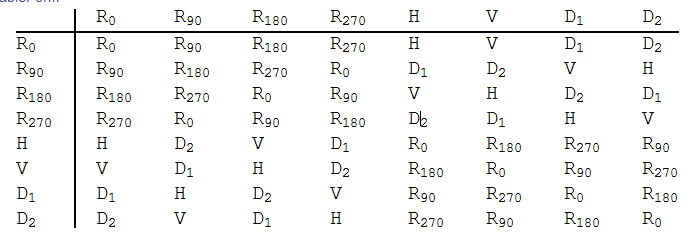
\includegraphics[width=\textwidth]{tableau_triangle.png}
        \caption{Tableau du groupe $\brace I/r_0, R_90, R_180, R_270, H, V, D_1,
        D_2 \rbrace$$, \circ$ représentant les relations entre les symétries du
        carré.}
        \label{fig:grptabl}
    \end{figure}


    \section{Divers}
    \subsection{Emsembles} \label{ss:jargondom}
    \subsection{Rappel division écrite}
    La multiplication de deux facteurs $a$ et $b$ donne un nombre dans lequel
    $a$ rentre $b$ fois (et inversément). Elle peut être vue comme une
    \emph{addition} répétée, la somme de $a$ nombre $b$.

    La division d'un nominateur $a$ et d'un dénominateur $b$ donne le nombre de
    fois que $b$ rentre dans $a$. Elle peut être vue comme une
    \emph{soustraction} répétée ; combien de fois on peut soustraire $b$ à $a$.

    On remarque tout de suite que ces deux opérations sont l'inverses l'une de
    l'autre. La multiplication additionne, la division soustrait. La
    multiplication donne le numérateur de la division à partir du dénominateur
    et du quotien.

    Ainsi, multiplier par $x$ revient à diviser par $x^{-1}$ (et inversément) et
    multiplier par $x$ puis divisé par $x$ reviens à ne rien faire.
    \begin{align*}
        a \cdot b &= c \\
        \frac{c}{b} &= a \\
        \frac{c}{a} &= b
    \end{align*}
    \subsection{Division polynomiale}
    \subsection{Lever la limite}
    \subsection{Produits remarquables}
    \subsection{Un nombre est divisible par x si...}
    \subsection{Exposants et racines}
    \subsection{Autres propriétés algébriques}

\end{document}